% TeX root = ../Main.tex

\section{Coleccion de datos}

En este trabajo, se realizaron filtrados y análisis de datos de partidos de fútbol correspondientes al año 2022 de la primera división del fútbol argentino. Este proceso se llevó a cabo en un entorno de Python utilizando Jupyter Notebook, lo que permitió la manipulación y visualización de los datos de manera eficiente. La colección de datos original abarcaba el período de 2015 a 2022, pero se focalizó en el año 2022 para obtener información actualizada y específica.

El objetivo principal de este análisis es la distribucion de goles por equipo en los partidos jugados durante el año 2022. Para lograrlo, se utilizaron técnicas y herramientas de programación en Python, lo que facilitó la extracción, filtrado y procesamiento de los datos correspondientes a ese año. Esto aseguró que los resultados obtenidos fueran relevantes y precisos en relación con el período de interés.




\section{Descripcion de la muestra}

Contiene la información de 2821 partidos de primera división del fútbol argentino agrupando datos de promeidos.com.ar, transfermarkt.de and oddportal.com en el archivo "afa.2015.2022.spa.csv"
\begin{itemize}
    \item torneo: nombre del torneo en curso cuando se jugó el partido. promiedos
    \item fecha: en qué fecha se jugó el partido. promiedos.
    \item partido: número de partido dentro de la fecha. promiedos.
    \item equipo\_local(visitante): nombre del equipo local(visitante) promiedos.
    \item goles\_local(visitante): número de goles anotados por el equipo local(visitante). promiedos.
    \item goles\_visitante(visitante): porcentaje de posesión del equipo local(visitante). promiedos.
    \item resultado: resultado del encuentro.
    \item fecha\_encuentro: fecha del encuentro. oddsportal.
\end{itemize}


\begin{figure}[h]
  \begin{center}
    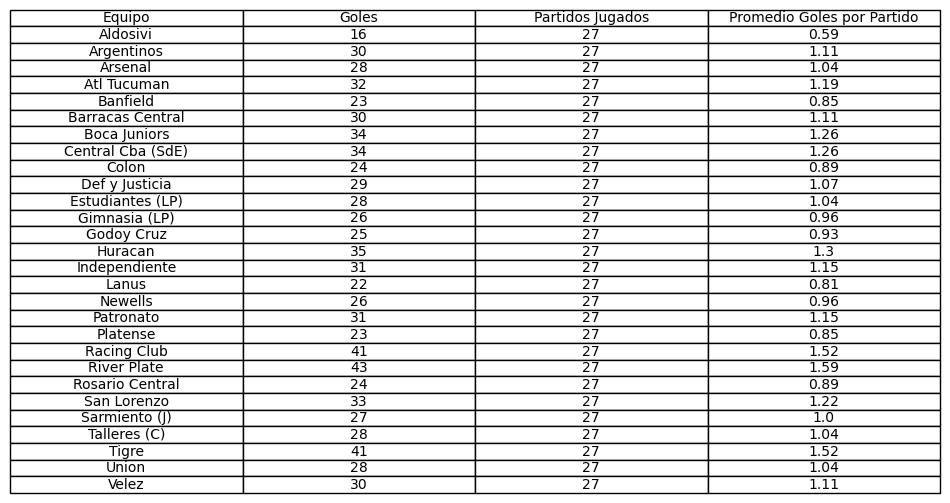
\includegraphics[width=0.75\textwidth]{/home/lucas/facultad/PyE/Promedio3.png}
   \caption{Tabla de promedio de goles.}
  \end{center}
\end{figure}

\begin{figure}[h]
  \begin{center}
    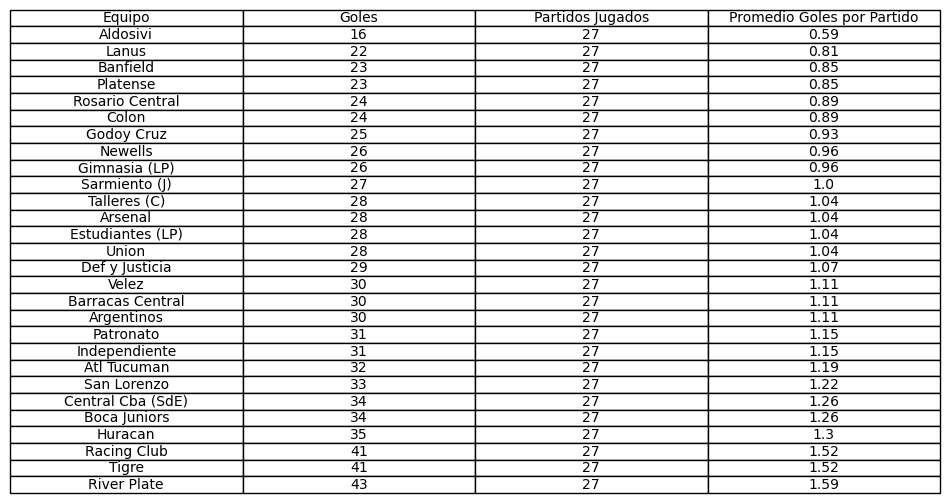
\includegraphics[width=0.72\textwidth]{/home/lucas/facultad/PyE/promediosOrdenados.png}
   \caption{Tabla de promedio de goles orden ascendente.}
  \end{center}
\end{figure}

\clearpage
\section{Grafico de caja}
\begin{align*}
\text{$Xmin$} &: \text{Valor mínimo dentro de los bigotes = 0.59} \\
\text{$Xmax$} &: \text{Valor máximo dentro de los bigotes = 1.59}
\end{align*}

\begin{figure}[h]
%\vspace{-10cm}
    \centering
    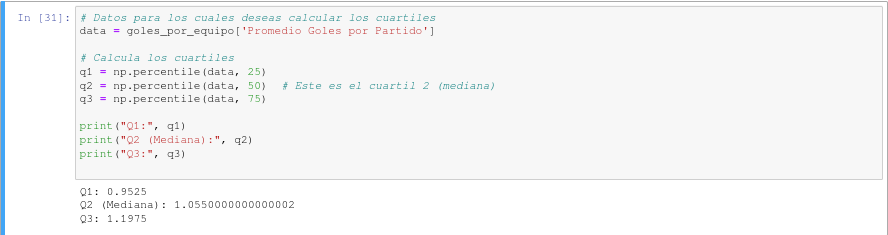
\includegraphics[width=0.9\textwidth]{/home/lucas/facultad/PyE/CalculoCuartiles.png}
    \caption{Calculo cuartiles.}
    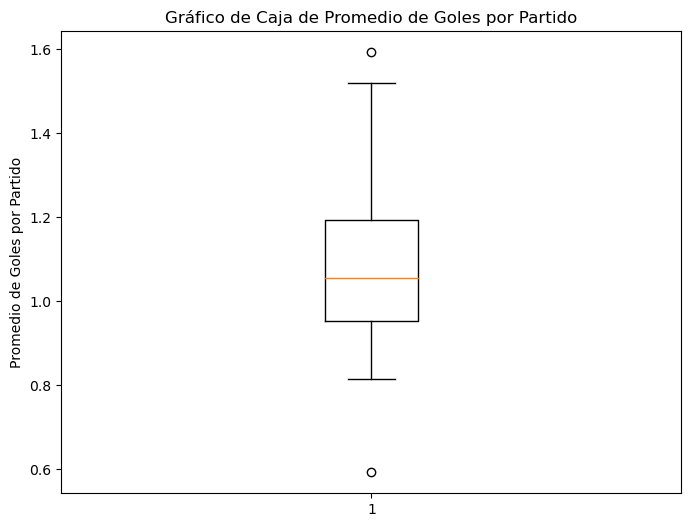
\includegraphics[width=0.7\textwidth]{/home/lucas/facultad/PyE/GraficoCaja.png}

\end{figure}

\section{Histograma}

Aquí está la tabla que muestra los límites de los intervalos, la frecuencia absoluta, la frecuencia relativa, la frecuencia acumulada y la frecuencia relativa acumulada del histograma:


\[
N_i = \sqrt{n}
\]

donde \(n\) es el número de observaciones en el conjunto de datos. En nuestro caso, \(n = 27\), por lo que:

\[
N_i = \sqrt{26} \approx 5
\]

Esto significa que aproximadamente necesitaremos 5 intervalos para construir nuestro histograma de manera efectiva.




%\vspace{-10cm}
\begin{figure}[h]
  \begin{center}
    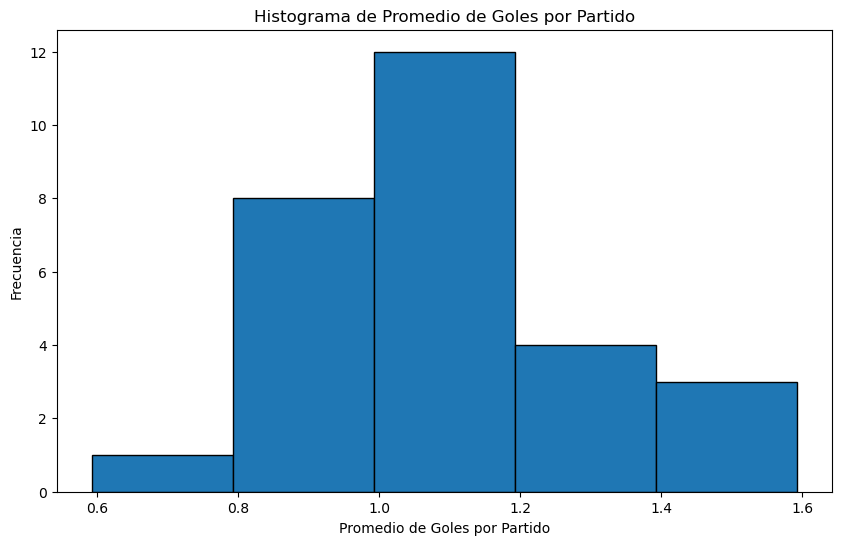
\includegraphics[width=0.95\textwidth]{/home/lucas/facultad/PyE/Histograma.png}
  \end{center}
\end{figure}




\begin{table}[h]
\centering
\begin{tabular}{|c|c|c|c|c|c|c|}
\hline
\textbf{Intervalo} & \textbf{Límite Inferior} & \textbf{Límite Superior} & \textbf{F abs} & \textbf{F rel} & \textbf{F rel acu} & \textbf{Fr acu} \\ \hline
1                  & 0.59                    & 0.79                    & 1             & 0.04          & 1             & 0.04            \\ \hline
2                  & 0.80                    & 0.99                    & 8             & 0.29          & 9             & 0.32            \\ \hline
3                  & 1.00                    & 1.19                    & 11            & 0.39          & 20            & 0.71            \\ \hline
4                  & 1.20                    & 1.39                    & 5             & 0.18          & 25            & 0.89            \\ \hline
5                  & 1.40                    & 1.59                    & 3             & 0.11          & 28            & 1.0             \\ \hline
\end{tabular}
\caption{la relacion de inclusion tomada para los intervalos es cerrada [inf;sup]}
\end{table}

\section{Gráficos}

\subsection{Polígono de Frecuencia}

Aquí se muestra el polígono de frecuencia:

\begin{figure}[h]
  \centering
  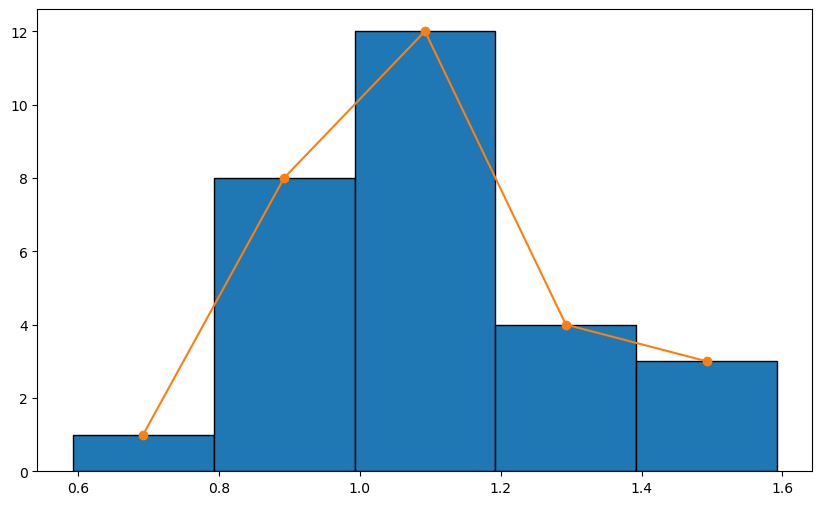
\includegraphics[width=0.7\textwidth]{/home/lucas/facultad/PyE/poligonoFrecuencia.png} % Reemplaza 'poligono_frecuencia.png' con el nombre de tu archivo de imagen
  \caption{Polígono de Frecuencia}
\end{figure}

\subsection{Ojiva de Frecuencia}

A continuación, se presenta la ojiva de frecuencia:

\begin{figure}[h]
  \centering
  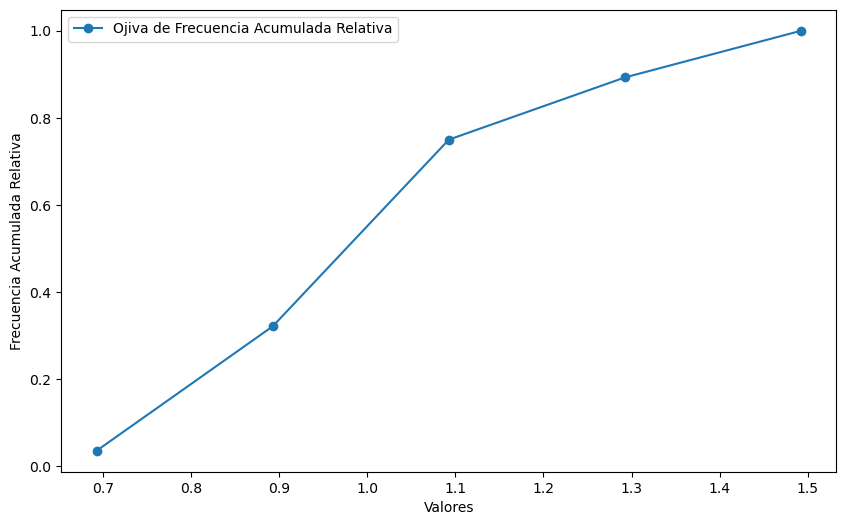
\includegraphics[width=0.7\textwidth]{/home/lucas/facultad/PyE/ojiva.png} % Reemplaza 'ojiva_frecuencia.png' con el nombre de tu archivo de imagen
  \caption{Ojiva de Frecuencia}
\end{figure}

\subsection{Gráfico de Torta}

Finalmente, el gráfico de torta correspondiente:

\begin{figure}[h]
  \centering
  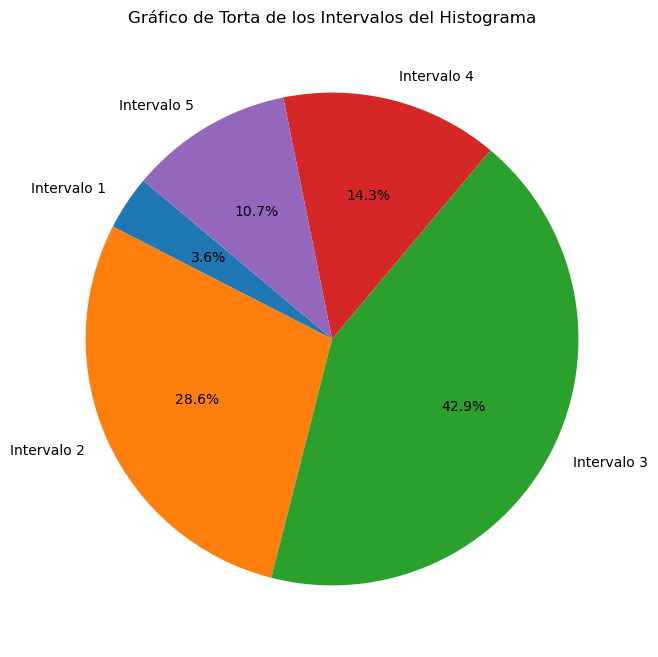
\includegraphics[width=0.5\textwidth]{/home/lucas/facultad/PyE/graficoTorta.png} % Reemplaza 'grafico_torta.png' con el nombre de tu archivo de imagen
  \caption{Gráfico de Torta}
\end{figure}

\section{Parametros}


$Promedio (Media): $X_{\text{prom}} = \frac{1}{n} \sum_{i=1}^{n} x_i$ = 1.09

$Desvío Estándar: $S = \sqrt{\frac{1}{n} \sum_{i=1}^{n} (x_i - X_{\text{prom}})^2}$ =0.2196

$Desvío Normal: $S_{n-1} = \sqrt{\frac{1}{n-1} \sum_{i=1}^{n-1} (x_i - X_{\text{prom}})^2}$ = 0.2236 

$Asimetria = \frac{\frac{1}{n} \sum_{i=1}^{n} (x_i - X_{\text{prom}})^3}{S^3}$ = 0.43

$Curtosis= \frac{\frac{1}{n} \sum_{i=1}^{n} (x_i - X_{\text{prom}})^4}{S^4}$ = 0.06

Moda: Valor(s) que aparece(n) con mayor frecuencia en los datos = 1.04

Cuartil 1 (Q1): $Q1 = x_{(n+1)/4}$ = 0.95

Cuartil 3 (Q3): $Q3 = x_{(3n+1)/4}$ = 1.19

En el apéndice, se pueden encontrar los detalles de los cálculos  (ver Apéndice \ref{ap:desviacion_estandar}).

\section{Estimacion}
En este apartado se calculará el error estándar, junto con intervalos de confianza para la esperanza y la varianza al 90 \%, 95\% y 99\%. Se estimará intervalos de confianza para la probabilidad a partir de la frecuencia relativa de los intervalos al 95\% y se estimará los intervalos de predicción al 90\%, 95\% y 99\%.




Siguiendo el concepto de error de medición donde \(x = x_0 \pm \Delta x\), a la hora de hacer cálculos con 26 datos distintos, como no se puede asegurar la normalidad, recurrimos a un concepto nuevo denominado “Error estándar”, tomando el mismo papel que \(\Delta x\), pero con un cálculo distintivo.

\[
E = \frac{s_{n-1}}{\sqrt{n}}
\]
Luego hay que encontrar lo que representa x0, 	que en este caso es el promedio calculado en un principio. 
Por lo tanto:

\[
x_0 \pm \Delta x = \bar{x} \pm  \frac{s_{n-1}}{\sqrt{n}} = 1,09 \pm 0.04 
\]

\subsection{intervalo de confianza}

Para calcular estos intervalos usaremos la teoría dada sobre la Aplicación de t de Student. La fórmula que se plantea es la siguiente 
\[
\(\bar{x} \pm t \left( \frac{s_{n-1}}{\sqrt{n}} \right)\)
\]
\[
 l_i = \bar{x} - t \left( \frac{s_{n-1}}{\sqrt{n}} \right)\)
\]
\[
 l_s = \bar{x} + t \left( \frac{s_{n-1}}{\sqrt{n}} \right)\)
\]
\[
  (l_i ; l_s)
\]

luego mediante codigo generado en python se obtuvo los siguientes resultados y el respectivo tamano:

Esperanza 90:
\[
 (1.015314327336203, 1.1592888472669718) 
\]
\[
  {T} = 0.1439745199307687 
\]

Esperanza 0.95:
\[
  (1.0005836522590859, 1.174019522344089)
\]
\[
  {T} = 0.17343587008500316 
\]

Esperanza 0.99:
\[
  (0.9702022933934336, 1.2044008812097413)
\]
\[
{T} = 0.23419858781630776 
\]

Ahora se calculara para la varianza utilizando la siguiente la formula dada por la distribución chi cuadrado, tendremos que calcular el equivalente al t del método t de student para buscar valores en la tabla


\[
\bar{x} \pm t_{\alpha/2} \left \frac{s_{n-1}}{\sqrt{n}} \
\]


Varianza 90:
\[
 (16.151395849664098, 40.113272069413625)
\]
\[
  {T} = 23.961876219749527
\]

Varianza 0.95:
\[
 (14.573382730821702, 43.19451096615604)
\]
\[
  {T} = 28.621128235334336 
\]

Varianza 0.99:
\[
  (11.807587351366145, 49.644915298994256)
\]
\[
{T} = 37.83732794762811
\]


luego queda calcular el Intervalo de confianza (probabilidad a partir de la frecuencia relativa al 95\%).
Para el siguiente calculo se utilizará la formula dada por el cálculo de Intervalo de confianza para una probabilidad a partir de una proporción, que en esencia es igual al de la probabilidad a partir de la frecuencia relativa al 95\%.

\[
\hat{p} = f_r mayor \%= 0,39
\]

\[
n = 26 (datos)
\]

\[
Z_{\frac{\alpha}{2}} = 1,96
\]
\[
\hat{p} \pm Z_{\frac{\alpha}{2}}\frac{\sqrt{\frac{\hat{p}(1-\hat{p}))}{n}+\frac{Z_{\frac{\alpha}{2}}^2{}}{4n^2}}}{1+\frac{Z_{\frac{\alpha}{2}}^2}{n}}
\]

Luego

\[
l_i = 0,55 
\]
\[
l_s = 0,21 
\]

Intervalo de Predicción (al 90\%):

A continuación, se implementará una formula conocida por teoría donde se plantea que
\[
\bar{x} \pm t_{n-1;\frac{\alpha}{2}}S_{n-1}\sqrt{1+\frac{1}{n}}
\]

\[
 t = 2,0452
\]
\[
  \bar{x}= 1,09
\]
\[
  S_{n-1} = 0.2236
\]
\[
t_1 = 1,708 
\]
\[
t_2  = 2.060
\]
\[
t_3 = 2.787
\]

luego obtenemos:

Intervalo de Predicción (al 90\%):
\[
 (0.70,1.47)
\]


Intervalo de Predicción (al 95\%):
\[
 (0.62,1.55)
\]

Intervalo de Predicción (al 99\%):
\[
 (0.45,1.72)
\]

% do a break page
\clearpage
\section{Segunda Muestra}


\begin{table}[h]
\centering
\begin{tabular}{|l|l|l|l|l|}
\hline
   & \textbf{Equipo}            & \textbf{Goles} & \textbf{Partidos Jugados} & \textbf{Promedio Goles por Partido} \\ \hline
2  & Arsenal           & 12    & 27               & 0.44                       \\ \hline
4  & Banfield          & 20    & 27               & 0.74                       \\ \hline
3  & Atl Tucuman       & 22    & 27               & 0.81                       \\ \hline
22 & Sarmiento (J)     & 23    & 27               & 0.85                       \\ \hline
21 & San Lorenzo       & 23    & 27               & 0.85                       \\ \hline
16 & Patronato         & 23    & 27               & 0.85                       \\ \hline
18 & Racing Club       & 24    & 27               & 0.89                       \\ \hline
15 & Newells           & 24    & 27               & 0.89                       \\ \hline
1  & Argentinos        & 26    & 27               & 0.96                       \\ \hline
7  & Colon             & 26    & 27               & 0.96                       \\ \hline
10 & Gimnasia (LP)     & 27    & 27               & 1.0                        \\ \hline
13 & Independiente     & 27    & 27               & 1.0                        \\ \hline
12 & Huracan           & 28    & 27               & 1.04                       \\ \hline
0  & Aldosivi          & 29    & 27               & 1.07                       \\ \hline
6  & Central Cba (SdE) & 30    & 27               & 1.11                       \\ \hline
24 & Union             & 32    & 27               & 1.19                       \\ \hline
25 & Velez             & 34    & 27               & 1.26                       \\ \hline
11 & Godoy Cruz        & 35    & 27               & 1.3                        \\ \hline
5  & Boca Juniors      & 35    & 27               & 1.3                        \\ \hline
17 & Platense          & 36    & 27               & 1.33                       \\ \hline
23 & Talleres (C)      & 38    & 27               & 1.41                       \\ \hline
20 & Rosario Central   & 39    & 27               & 1.44                       \\ \hline
9  & Estudiantes (LP)  & 43    & 27               & 1.59                       \\ \hline
8  & Def y Justicia    & 43    & 27               & 1.59                       \\ \hline
14 & Lanus             & 44    & 27               & 1.63                       \\ \hline
19 & River Plate       & 53    & 27               & 1.96                       \\ \hline
\end{tabular}
\caption{promedio de goles por equipo en la temporada 2021}
\end{table}

% continuar en la proxima pagina y agregar imagen del histograma2021

\breakpage
\begin{figure}[h]
  \begin{center}
    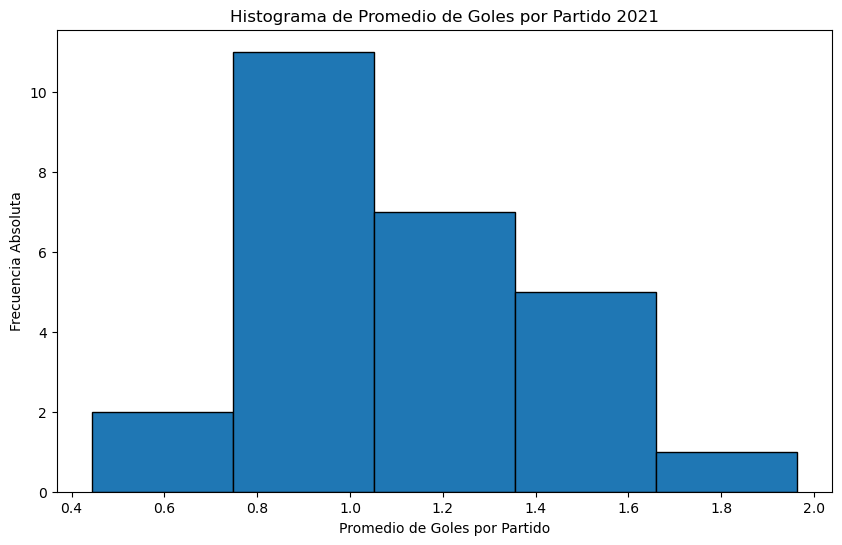
\includegraphics[width=0.95\textwidth]{/home/lucas/facultad/PyE/histograma2021.png}
  \end{center}
\end{figure}

se obtiene que:


% hacer subsecciones para media, desvio normal, Intervalo de confianza para la esperanza (al 95%) y Intervalo de confianza para la varianza (al 95%).
\subsection{Media}
\[
\bar{x}=1.13
\]

\subsection{Desvio Normal}
% desvio normal
\[
S_{n-1} = 0.33
\]

\subsection{Intervalo de confianza para la esperanza (al 95\%)}
\[
\(\bar{x} \pm t \left( \frac{s_{n-1}}{\sqrt{n}} \right)\)
\]
\[
 l_i = \bar{x} - t \left( \frac{s_{n-1}}{\sqrt{n}} \right)\) = 1.0005
\]
\[
  l_s = \bar{x} + t \left( \frac{s_{n-1}}{\sqrt{n}} \right)\) = 1.1740
\]

\subsection{Intervalo de confianza para la varianza (al 95\%)}
\[
\bar{x} \pm t_{\alpha/2} \left \frac{s_{n-1}}{\sqrt{n}} \
\]

\[
 l_i = 14.57
\]
\[
 l_s = 43.19
\]

% crear secccion evaluacion de hipotesis
\section{Evaluacion de hipotesis}

se toma como evaluacion de hipotesis nula $(H_0)$ $\mu_0= 1.05$  que es el promedio redondeado hacia abajo y como hipotesis alternativa $(H_1)$ $\mu_1 = 1.09$ que representa el resultado del promedio de la primera meuestra
\[
  N\sim (\mu0 = \bar{x}; \sigma = S_{n-1}^2)
\]
\[
S_{n-1} = 0.22
\]
luego para H_0 se obtiene que:
\[
  N\sim (\mu0 = 1.05; \sigma = 0.04)
\]

y por ultimo H_1 se obtiene que:
\[
  N\sim (\mu1 = 1.09; \sigma = 0.04)
\]

dado un nivel de significacion $\alpha$, se calcula el limte de aceptacion haciendo uso de la siguiente formula:

\[
L = \mu0 + Z_a \frac{\sigma}{\sqrt{n}}
\]

Después, conociendo el valor de L, se puede calcular el error de cometer un error de tipo 2
haciendo uso de la siguiente fórmula:
\[
  \beta = P(Z = \frac{\bar{X-\mu1}}{\frac{\sigma}{\sqrt{n}}}\leq \frac{L-\mu1}{\frac{\sigma}{\sqrt n}}=Z_L) = P(Z\leq Z_L)=\phi(Z_L)=\phi(\frac{\bar{X-\mu1}}{\frac{\sigma}{\sqrt{n}}})  
\]
\begin{table}[h]
  \centering
  \begin{tabular}{|c|c|c|c|}
  \hline
  \textbf{Nivel de Significancia} & \textbf{Z\textsubscript{a}} & \textbf{L} & \textbf{$\beta$} \\
  \hline
  1\%                               & 2.327                       & 1.15      & 91\%        \\
  5\%                               & 1.645                       & 1.12      & 75\%      \\
  10\%                              & 1.285                       & 1.10      & 59\%        \\
  \hline
  \end{tabular}
  \end{table}
  
\subsection{Límites de aceptación a dos colas}
\[
  L_i = \mu0 - Z_a \frac{\sigma}{\sqrt{n}}
  \]
  \[
    L_s = \mu0 + Z_a \frac{\sigma}{\sqrt{n}}
    \]
Y similarmente, el cálculo de el riesgo de cometer un error del tipo 2 se calcula de la
siguiente forma
\[
  \beta = \phi(Z_l_s)-\phi(Z_l_i)
\]






%
% \appendix
% \label{ap:desviacion_estandar}
% \section{Apéndice: Detalles de los Cálculos}
% \subsection{Cálculo de parametros}
% \begin{figure}[h]
%   \vspace{-8cm}
%   \centering
%   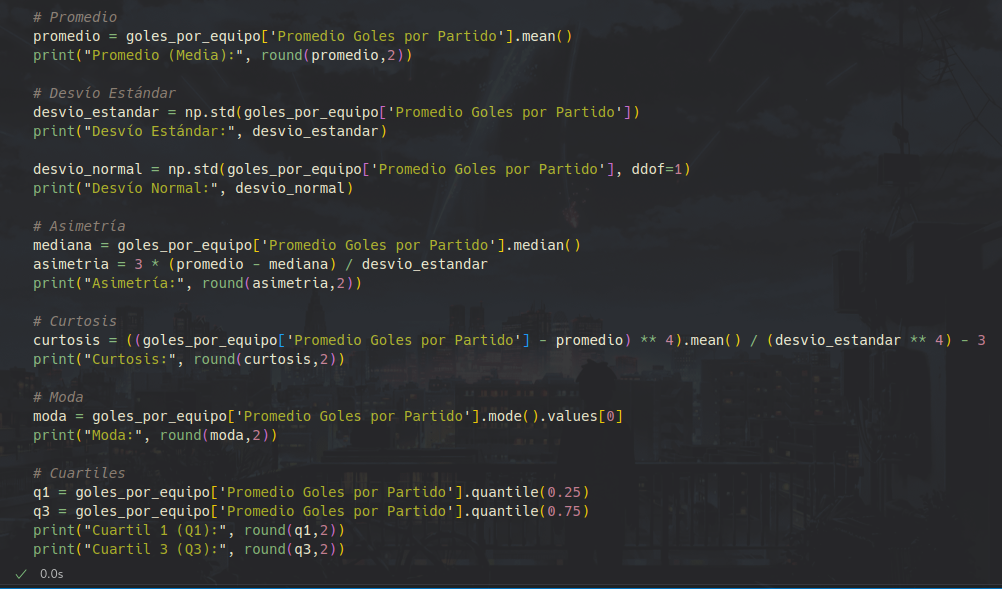
\includegraphics[width=0.8\textwidth]{/home/lucas/facultad/PyE/calculo1.png} 
%   \caption{Codigo}
%   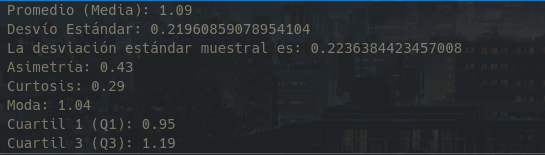
\includegraphics[width=0.8\textwidth]{/home/lucas/facultad/PyE/calculo2.png} 
%   \caption{Output}
%
% \end{figure}
